\documentclass[oldfontcommands,oneside,a4paper,11pt]{article} 
\usepackage{fontspec}
\usepackage{natbib}
\usepackage{booktabs}
\usepackage{xltxtra} 
\usepackage{longtable}
\usepackage{polyglossia} 
\usepackage[table]{xcolor}
\usepackage{lineno}
\usepackage{gb4e} 
\usepackage{multicol}
\usepackage{graphicx}
\usepackage{float}
\usepackage{hyperref} 
\hypersetup{bookmarks=false,bookmarksnumbered,bookmarksopenlevel=5,bookmarksdepth=5,xetex,colorlinks=true,linkcolor=blue,citecolor=blue}
\usepackage[all]{hypcap}
\usepackage{memhfixc}
\usepackage{lscape}
\usepackage{lineno}
\bibpunct[: ]{(}{)}{,}{a}{}{,}
%%%%%%%%%quelques options de style%%%%%%%%
%\setsecheadstyle{\SingleSpacing\LARGE\scshape\raggedright\MakeLowercase}
%\setsubsecheadstyle{\SingleSpacing\Large\itshape\raggedright}
%\setsubsubsecheadstyle{\SingleSpacing\itshape\raggedright}
%\chapterstyle{veelo}
%\setsecnumdepth{subsubsection}
%%%%%%%%%%%%%%%%%%%%%%%%%%%%%%%
%\setmainfont[Mapping=tex-text,Numbers=OldStyle,Ligatures=Common]{Charis SIL} 
\newfontfamily\phon[Mapping=tex-text,Ligatures=Common,Scale=MatchLowercase,FakeSlant=0.3]{Charis SIL} 
\newcommand{\ipa}[1]{{\phon \mbox{#1}}} %API tjs en italique
 
 
 
\newcommand{\grise}[1]{\cellcolor{lightgray}\textbf{#1}}
\newfontfamily\cn[Mapping=tex-text,Ligatures=Common,Scale=MatchUppercase]{MingLiU}%pour le chinois
\newcommand{\zh}[1]{{\cn #1}}

\newcommand{\jg}[1]{\ipa{#1}\index{Japhug #1}}
\newcommand{\wav}[1]{#1.wav}
\newcommand{\tgz}[1]{\mo{#1} \tg{#1}}

\XeTeXlinebreaklocale 'zh' %使用中文换行
\XeTeXlinebreakskip = 0pt plus 1pt %
 %CIRCG
\begin{document} 

\title{Tonogenesis and tonal alternations in Khaling\footnote{I would like to thank Aimée Lahaussois, Jean-Léo Léonard,  Boyd Michailovsky and Enrique Palancar  for useful comments on previous version of this work. I am responsible for any remaining error. Abbreviation follow the Leipzig glossing rules, except for the following: C consonant V vowel, \textsc{di} / \textsc{pi} dual / plural inclusive \textsc{de} / \textsc{pe} dual / plural exclusive.}}
\author{Guillaume Jacques }
\maketitle
\linenumbers

\sloppy


\textbf{Abstract}: In this paper, we present a historical account for the tonal alternations observed in the Khaling verbal system. We show that most of these alternations can be explained by two series of sound change. First, level and falling tones   appeared in closed syllables with sonorant and obstruents codas respectively. Second, the loss of vowel in specific contexts   lead to the development of additional falling tones. A residue of falling tones remain unaccounted for by the present reconstruction, but several hypotheses are proposed to explain their origin.

\textbf{Keywords}: Tonogenesis, Syllable reduction, Obstruents, Kiranti, Khaling
 
 \section{Introduction}
Khaling,\footnote{Khaling is spoken by around 15000 speakers in Solukhumbu district, Nepal, see Figure \ref{fig:kiranti}.} like other Kiranti languages, has a very complex templatic verbal morphology (see for instance \citealt{bickel07chintang} and \citealt{jacques12agreement}). It is unique in the Kiranti subgroup however in having relatively recently innovated a tonal system.\footnote{Tonogenesis and most vowel changes postdate the start of Nepali influence in the eighteenth century, as will be shown in section \ref{sec:obstruents}.} 


\begin{figure}[h]
\centering
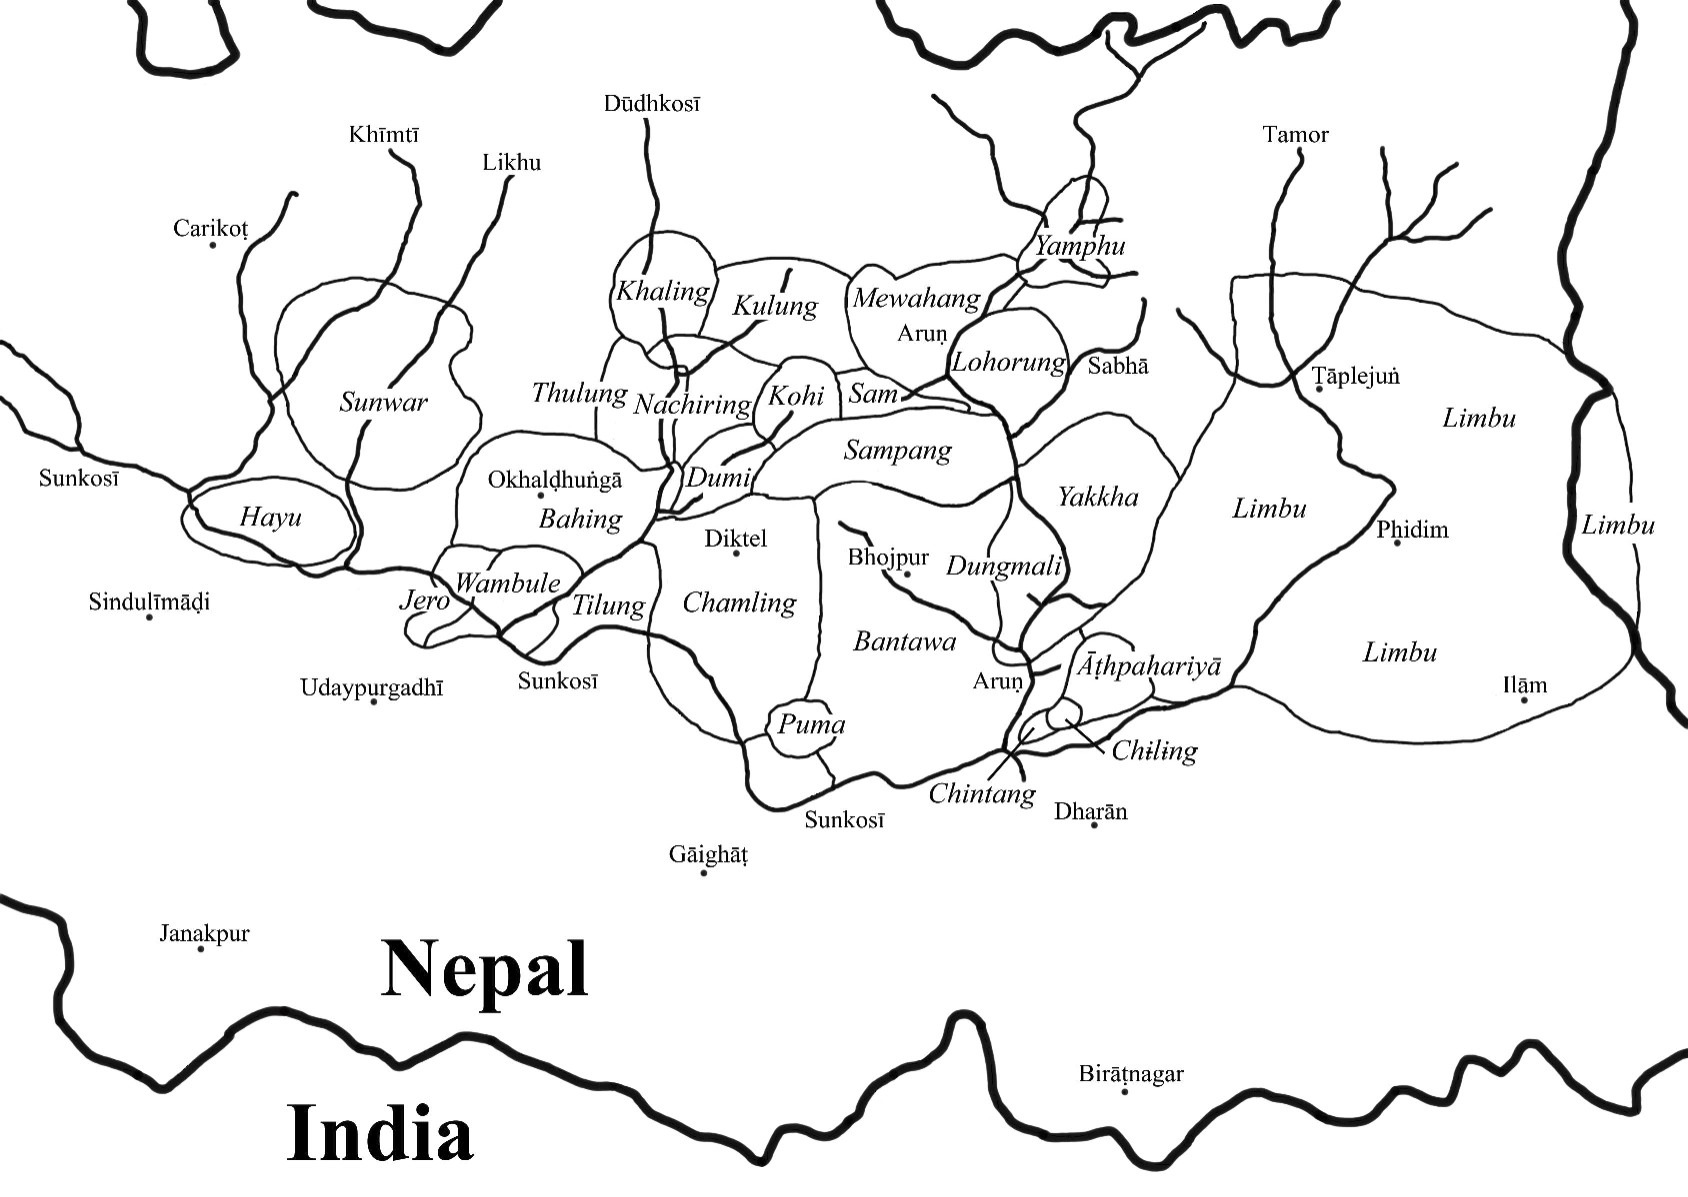
\includegraphics[height=100mm]{Kirant.jpeg}
\caption{Map of Kiranti languages (from \citealt{opgenort11tilung})}
\label{fig:kiranti}
\end{figure}


 Tone in Khaling is not only phonemic in that it is used to distinguish between lexical minimal pairs, it also plays a critical role  the structure of the verbal inflectional system of the language. Complex patterns of stem alternation involving vowel, consonant and tonal changes are observed in this language. These alternations are not correlated in isomorphic fashion with any morphosyntactic feature.  The distribution of stems (and of tonal alternations) in the Khaling verbal system is influenced by transitivity, person and number of one or two arguments, tense (past vs non-past) in an intricate way. The complete list of conjugation classes, as well as a computational model to automatically generate them is provided in \citet{jacques12khaling}. The conjugation classes with the greatest number of stems has up to ten of them, while those with the fewest number of stems only have two (but such classes are very limited).

Table \ref{tab:intro} illustrate some typical examples of stem alternations. All the forms in the table comprise a stem followed by one unstressed short vowel suffix (which has no tonal contrast). These data show that while in some verb conjugation classes the tone is constant in all stems (for instance, in the case of the verb `jump' we have level tone, indicated by a macron, in all forms), in most conjugation classes we observe alternations between falling tone (marked with a retroflex accent) and level tone (with a macron, see the conjugation of `touch') or between falling tone and short vowel syllables where the tonal contrast is neutralized (`go' and `hit'). 

Table \ref{tab:intro} also illustrates the fact that tonal alternations in Khaling are not completely independent of vowel and final consonant alternations: in the case of the verb `touch' for instance, the see that the level tone is correlated with the stem final consonants \ipa{--j} and \ipa{--ʦ}, while the falling tone appears in stems with final \ipa{--n}.


\begin{table}[h]
\caption{Examples of tonal alternations in the Khaling verbal system} \centering \label{tab:intro}
\begin{tabular}{llllll}
\toprule
Infinitive & Non-past \textsc{1di} & Non-Past \textsc{3pl} & Past \textsc{3sg} & Meaning \\
\midrule
\ipa{bʰoɔ̄j-nɛ} &	\ipa{bʰɵ̄ːʦ-i} &	\ipa{bʰoɔ̂n-nu} &	\ipa{bʰoɔ̂n-tɛ} &	touch	(tr) \\
\ipa{ʦoɔ̄j-nɛ} &	\ipa{ʦɵ̄ːʦ-i} &	\ipa{ʦoɔ̄j-nu} &	\ipa{ʦɵ̄ːs-tɛ} &	jump	(intr) \\
\ipa{kʰoɔ̂n-nɛ} &	\ipa{kʰɵʦ-i} &	\ipa{kʰoɔ̂n-nu} &	\ipa{kʰɵs-tɛ} &	go	(intr) \\
\ipa{roɔ̂n-nɛ} &	\ipa{rɵʦ-i} &	\ipa{rɵ̂ːt-nu} &	\ipa{rɵ̂ː-tɛ} &	hit	(intr) \\
\bottomrule
\end{tabular}
\end{table}

In addition, we observe that stem distribution and tonal alternation cannot be accounted for by a single factor. \citet{walther14compactness} has shown that stem alternations is Khaling is better accounted for by a morphomic account, rather than in terms of transparent morphosyntactic features. 

The apparent chaos of verb stem alternations in general, and the opacity of tonal alternations in particular, can however be partially accounted for  by a historical account based on a combined application of the comparative method and of internal reconstruction. Most of the tonal alternations in Khaling can be straightforwardly explained as the mechanical result of two major sources of tonal contrasts: the transphonologization of stem final consonant contrasts into tonal contrasts, and the creation of falling tones following the loss of some final syllables.

Given the fact that tonal alternations are not completely independent from segmental changes in Khaling, it is necessary to opt for an approach that does not treat tones in isolation from vowel and consonants, and therefore part of the paper will provide the minimal quantity of information on segmental alternations and their origins that are necessary to make sense  of the tonal alternations.

First, we describe  Khaling synchronic phonology, including segmental inventories, phonotactic rules and tonal contrasts. 
 
Second, we present a simplified picture of stem alternations in Khaling,\footnote{For reasons of space, since the present paper is focused on tone, this section is limited to the strict minimum necessary to follow the tonogenesis model. An exhaustive account of alternations can be found in \citet{jacques12khaling}.} and propose to reconstruct a stress pattern in pre-Khaling to account for vowel lengthening in some stem types. Although this section does not directly discuss tonal alternations in Khaling, it is a pre-requisite for the complete tonogenesis model elaborated in the following section.
 
Third, we provide a detailed account of tonogenesis in Khaling. Although a partial discussion of the origin of tones can be found in \citet{michailovsky75khaling}, the present paper, based on more reliable and complete data, shows that tones in Khaling have more than one origin and describes for the first time the development of falling tones correlated with the loss of final vowels. Some sound laws are demonstrated on the basis of data from nouns rather than verbs, to avoid circularity in the internal reconstruction of the verbal system.

Fourth, we show how the model of tonogenesis proposed in the previous section can account for most tonal alternations in the Khaling verbal system. Pre-Khaling as reconstructed in this model was more similar to other Kiranti languages in having a less elaborate system of stem alternation, and suprasegmentals were restricted to stress shifts.

Fifth, we point out the presence of a residue of forms which cannot be explained as the result of regular sound changes using the laws elaborated in the tonogenesis section. Several potential lines of explanation involving analogical leveling are explored.

\section{Synchronic phonology} \label{sec:synchr}

As shown in \citet[1098]{jacques12khaling}, Khaling has eighteen vowel  phonemes (Table \ref{tab:vowels}) and 27 consonant phonemes (Table \ref{tab:consonants}). The only word-initial clusters allowed are labial or velar stop + \ipa{l} and \ipa{r}. 

The consonant \ipa{ç} only appears as the first element of a word-internal cluster (as in \ipa{seçki} `we kill it'), never word-initially or word-finally. Only unvoiced obstruents and sonorants \ipa{--p}, \ipa{--t} \ipa{--k}, \ipa{--m}, \ipa{--n}, \ipa{--ŋ}, \ipa{--r}, \ipa{--l}, \ipa{--s} and \ipa{--j} can occur as codas. Clusters involving two unvoiced stops or affricates (such as \ipa{pt}, \ipa{kt} etc), as well as geminates (\ipa{tt}, \ipa{pp}, \ipa{kk} and \ipa{ʦʦ}), are realized with preaspiration when the preceding vowel is short.

Unique among Sino-Tibetan languages, Khaling has a contrast between simple stop codas and geminated stop codas, realized as preaspirated final consonants as in \ipa{pɛpp} [pʲɛʰp] `father'  or \ipa{pʰɛtt} [pʰʲɛʰt] `egg'. Th diphthong \ipa{oɔ} is treated a a unique phoneme.

\begin{table}[H]
\caption{List of Khaling vowel phonemes} \label{tab:vowels}\centering
\begin{tabular}{llllll}
\ipa{i iː} & \ipa{ʉ ʉː} & &&\ipa{u uː} \\
\ipa{e eː} & \ipa{ɵ ɵː} & &&\ipa{o oː} \\
\ipa{ɛ ɛː} &   & &\ipa{ʌ} &  \ipa{oɔ} \\
&&\ipa{a aː}\\
\end{tabular}
\end{table}

\begin{table}[H]
\caption{List of Khaling consonantal phonemes} \label{tab:consonants}\centering
\begin{tabular}{llllll}
\ipa{p} & \ipa{t} &&\ipa{ʦ}  & \ipa{k}&\ipa{ʔ}\\
\ipa{pʰ} & \ipa{tʰ} &&\ipa{ʦʰ}  & \ipa{kʰ}&\\
\ipa{b} & \ipa{d} &&\ipa{ʣ}  & \ipa{g}&\\
\ipa{bʰ} & \ipa{dʰ} &&\ipa{ʣʰ}  & \ipa{gʰ}&\\
\ipa{m} & \ipa{n} && & \ipa{ŋ}&\\
  & \ipa{s} && \ipa{ç}& &\ipa{ɦ}\\
  \ipa{w} & \ipa{l} &\ipa{r}&\ipa{j}  & &\\
\end{tabular}
\end{table}

Khaling has a two-way tonal contrast on open syllables with long vowels or closed syllables with a sonorant coda. There is a high level tone (indicated by a macron)\footnote{We opt for the macron rather than the acute accent for transcribing the level tone, as the acute accent is used in this paper for indicating stress in (non-tonal) pre-Khaling reconstruction, and we want to avoid confusion.} and a falling tone (circumflex accent). A marginal contrast between surface low level and high level tone is also attested in a very restricted morphosyntactic environment (see below), but it is irrelevant for the description of verbal flexion and its phonological interpretation is deferred to future research.

 The tonal contrast is neutralized  on short  and / or unstressed vowels. Note that in sonorant-final syllables, vowels are always long, and vowel length is not indicated as it is redundant. Table \ref{tab:minimal.pairs} illustrates possible tonal contrasts on monosyllables.  

In polysyllables, only stressed syllables receive tone, and verbs and nouns alike only have one stressed syllable, except in the case of compound verbs, which are not discussed in this paper.

\begin{table}[H]
\caption{Minimal pairs between level tone and falling tone in monosyllables } \label{tab:minimal.pairs}\centering
\begin{tabular}{llllll}
\toprule
Form & Meaning\\
\midrule
\ipa{mɛ̄m} & he \\
\ipa{mɛ̂m} & mother\\
\midrule
\ipa{mɛ̄ː} & there\\
\ipa{mɛ̂ː} & (ideophone) rolling quickly \\
\ipa{mɛ} & that\\
\bottomrule
\end{tabular}
\end{table}

In addition, a contrast between high level tone and a phonetically low tone is attested in the purposive construction with the locative suffix \ipa{-bi} followed by a motion verb. Verbs  whose root ends in a sonorant consonant \ipa{m}, \ipa{n}, \ipa{ŋ}, \ipa{l} or \ipa{r} use the infinitive stem with level tone before the locative suffix \ipa{--bi} as in example \ref{ex:cow}. Root-final   \ipa{--n} changes to \ipa{--j} in this context. 

\begin{exe}
\ex \label{ex:cow}
\gll \ipa{bʌ̂j} \ipa{ʔu-gʰas} \ipa{kɛ̄m-bi} \ipa{kʰɵs-tɛ}  \\
cow \textsc{3sg.poss}-grass chew-\textsc{loc} go-\textsc{pst:3sg} \\
\glt `The cow went to chew the grass.'
\end{exe}

Verbs with roots ending in obstruents use the nasalized infinitive stem (with final \ipa{--n} or \ipa{--ŋ} respectively) with falling tone in this construction.

Noun  and verb forms with falling tone  remain unchanged as in \ref{ex:elk}: the free noun `elk' \ipa{kɛ̂m} has the same form as when occurring with the locative suffix.

\begin{exe}
\ex \label{ex:elk}
\gll   \ipa{kɛ̂m-bi} \ipa{kʰɵs-tɛ}  \\
elk-\textsc{loc} go-\textsc{pst:3sg} \\
\glt `He went (to hunt) for the elk.'
\end{exe}


Monosyllabic nouns with level tone, however, develop a low tone in the purposive construction when suffixed by \ipa{-bi}, as \ipa{kɛ̄m}  `work'\footnote{Borrowed from Nepali \ipa{kam}.} in example \ref{ex:work}.
\begin{exe}
\ex \label{ex:work}
\gll   \ipa{kɛ̀m-bi} \ipa{kʰɵs-tɛ}  \\
work-\textsc{loc} go-\textsc{pst:3sg} \\
\glt `He went for his work.'
\end{exe}


This highly restricted, syntactically determined low alternant of the level tone will not be considered further in the present paper, as its synchronic analysis in still unclear (in particular, it remains to be determined whether a similar contrast is found in other grammatical constructions), and it is not necessary to the analysis of the verbal morphology.


In the following, we show the origin of the tonal and length contrasts in Khaling. We point  two origins for the falling tone: loss of obstruent codas and syllable reduction.

\section{Vowels and stress in pre-Khaling}

Although this paper focuses on the origin of the Khaling tonal system, it is necessary at this stage to provide a comparative account of Khaling historical phonology, since previous publications have only treated this topic from the point of view of internal reconstruction. In this section, we provide a justification for the reconstructions used in the following sections,   in particular   for the stress patterns reconstructed for pre-Khaling, which have a direct effect on tonogenesis.

Previous scholarship on comparative proto-Kiranti (\citealt{driem90r}, \citealt{michailovsky94stops}, \citealt{starostin94kiranti}, \citealt{opgenort05jero}) has focused on the reconstruction of proto-Kiranti consonants, but no work has been published on the vowel correspondences between Khaling and other Kiranti languages. In Khaling, as we will see, the evolution of vowels, codas and the development of tonal contrasts are closely related, so that an account of the basic vocalic sound laws is necessary for any further work on the topic.

%distinguish pre-Khaling 1 and pre-khaling 2, too early to provide proto-kiranti or even proto-khaling-dumi reconstructions
Internal reconstruction suggests that the complex vowel system of Khaling was innovated from a simpler vowel system, as can be ascertained from the vowel alternations in the verbal system and the complementary distributions between vowels and codas (\citealt{michailovsky75khaling}, \citealt{jacques12khaling}). 

As shown in \citet{michailovsky75khaling}, \citet{jacques12khaling} and \citet{michailovsky12dumi} using internal reconstruction, in both Khaling and Dumi, no more than five vowels have to be postulated in verbal roots. Complex morphophonological alternations yield all 18 vowels in different contexts. Table \ref{tab:basic.alternations} illustrates  the most important alternations: closed syllable  verb stems can be classified into two major categories, weak and strong. Weak stems are found mainly in forms with vowel initial suffixes (the exceptions are shown in Tables \ref{tab:intrans.paradigm}, \ref{tab:trans.paradigm} and \ref{tab:trans.cvct.paradigm} and discussed in section \ref{sec:tonogenesis.verb}), and strong stems are  found with consonant-initial suffixes except in the case of verb stems with final clusters, which always have \ipa{t} as second element (see the conjugation of CVCt roots in Table \ref{tab:trans.cvct.paradigm} and the discussion in section \ref{sec:cvct}).

\begin{table}[H]
\caption{Basic vowel alternations in the Khaling verb } \label{tab:basic.alternations} \centering
\begin{tabular}{lllllllll}
\toprule
 root vowel & 	open   & 	velar  & 	velar  & 	non-velar    & 	non-velar   \\
& syllable&(strong) &(weak) &(strong) &(weak) \\
\midrule
\ipa{a}  & 	\ipa{ɛ}  & 	\ipa{a}  & 	\ipa{ʌ}  & 	\ipa{ɛ}  & 	\ipa{ɛ}  \\ 	
\ipa{e}  & 	\ipa{e}  & 	\ipa{e}  & 	\ipa{e}  & 	\ipa{e}  & 	\ipa{e}  \\ 	
\ipa{i}  & 	\ipa{e}  & 	\ipa{ʌ}  & 	\ipa{i}  & 	\ipa{ʌ}  & 	\ipa{i}  \\ 	
\ipa{o}  & 	\ipa{ɵ}  & 	\ipa{o}  & 	\ipa{ɵ}  & 	\ipa{oɔ}  & 	\ipa{ɵ}  \\ 	
\ipa{u}  & 	\ipa{ʉ}  & 	\ipa{u}  & 	\ipa{ʉ}  & 	\ipa{ʌ}  & 	\ipa{ʉ}  \\ 	
\bottomrule
\end{tabular}
\end{table}

Some stem forms (\textsc{3sg:n.pst$\rightarrow$3sg} and \textsc{3sg:n.pst$\rightarrow$3sg}) have a lengthened vowel (see Table \ref{tab:basic.alternations.ex}), which we interpret as reflecting radical stress (vs suffixal stress) in pre-Khaling. Reconstructing stress for pre-Khaling has other important consequences, in particular for the Syllable Reduction Rule (section \ref{sec:disyll}).

\begin{table}[H]
\caption{Examples of basic vowel alternations in the Khaling verb } \label{tab:basic.alternations.ex} \centering
\resizebox{\columnwidth}{!}{
\begin{tabular}{lllllllll}
\toprule
Root& Meaning &   weak stem& weak stem (lengthened)& strong stem  &\\
&&(\textsc{1di:n.pst$\rightarrow$3sg})&(\textsc{3sg:n.pst$\rightarrow$3sg}) &\textsc{1pi:n.pst$\rightarrow$3sg}\\
\midrule
 |\ipa{pʰrok}|  & untie &\ipa{pʰrɵk-i}& \ipa{pʰrɵ̄ːg-ʉ} & \ipa{pʰrok-ki} \\
 |\ipa{lom}|  & search &\ipa{lɵm-i}& \ipa{lɵ̄ːm-ʉ} & \ipa{loɔ̄m-ki} \\
 |\ipa{lop}| & catch &\ipa{lɵp-i} &  \ipa{lɵ̄ːb-ʉ} & \ipa{loɔ̄p-ki} \\
 \bottomrule
\end{tabular}}
\end{table}


Tables \ref{tab:intrans.paradigm}, \ref{tab:trans.paradigm} and  \ref{tab:trans.cvct.paradigm} illustrate the distribution of the stems in the Khaling verbal paradigms. Irregular cases, where a weak stem is found with a consonant-initial suffix, are shaded in grey. These tables only represent   the stem vowel alternations, and do not include information on   consonant shifts, which are not the focus of the present paper (some such cases are treated in section \ref{sec:obstruents}). In addition to weak and strong stems, we also find lengthened weak stems in the transitive CVC paradigm.

\begin{table}[H]
\caption{Distribution of  stems in the intransitive paradigm } \label{tab:intrans.paradigm} \centering
\resizebox{\columnwidth}{!}{
\begin{tabular}{llllllll}
\toprule
S    &   	 non-past    &   	   &   	 past    &   	   &   	 imperative   &   	   &   	\\
\midrule
\textsc{1s}    &   	 strong-\ipa{ŋʌ}    &   	\ipa{ŋôŋ-ŋʌ}    &   	 weak-\ipa{ʌtʌ}    &   	\ipa{ŋɵk-ʌtʌ}   &   	   &   	   &   	\\
\textsc{1di}    &   	 weak-\ipa{i}    &   	\ipa{ŋɵk-i}   &   	 weak-\ipa{iti}    &   	\ipa{ŋɵk-iti}   &   	   &   	   &   	\\
\textsc{1de}    &   	 weak-\ipa{u}    &   	\ipa{ŋɵk-u}   &   	 weak-\ipa{utu}    &   	\ipa{ŋɵk-utu}   &   	   &   	   &   	\\
\textsc{1pi}    &   	 strong-\ipa{ki}    &   	\ipa{ŋok-ki}   &   	 strong-\ipa{tiki}    &   	\ipa{ŋok-tiki}   &   	   &   	   &   	\\
\textsc{1pe}    &   	 strong-\ipa{kʌ}    &   	\ipa{ŋok-kʌ}   &   	 strong-\ipa{tʌkʌ}    &   	\ipa{ŋok-tʌkʌ}   &   	   &   	   &   	\\
\textsc{2s}    &   	 \ipa{ʔi}-strong    &   	\ipa{ʔi-ŋôː}   &   	 \ipa{ʔi}-weak-\ipa{tɛ} \grise{}    &   	\ipa{ʔi-ŋɵk-tɛ}\grise{}   &   	weak-\ipa{je}\grise{}   &   	\ipa{ŋɵk-je} \grise{}  &   	\\
\textsc{2d}    &   	 \ipa{ʔi}-weak-\ipa{i}    &   	\ipa{ʔi-ŋɵk-i}   &   	 \ipa{ʔi}-weak-\ipa{iti}    &   	\ipa{ʔi-ŋɵk-iti}   &   	weak-\ipa{ije}    &   	\ipa{ŋɵk-ije}   &   	\\
\textsc{2p}    &   	 \ipa{ʔi}-strong-\ipa{ni}    &   	\ipa{ʔi-ŋôː-ni}   &   	 \ipa{ʔi}-weak-\ipa{tɛnu}\grise{}    &   	\ipa{ʔi-ŋɵk-tɛnu} \grise{}  &   	weak-\ipa{nuje}\grise{}   &   	\ipa{ŋɵk-nuje} \grise{}  &   	\\
\textsc{3s}    &   	 strong    &   	\ipa{ŋôː}   &   	 weak-\ipa{tɛ} \grise{}   &   	\ipa{ŋɵk-tɛ}  \grise{} &   	   &   	   &   	\\
\textsc{3d}    &   	 weak-\ipa{i}    &   	\ipa{ŋɵk-i}   &   	 weak-\ipa{iti}    &   	\ipa{ŋɵk-iti}   &   	   &   	   &   	\\
\textsc{3p}    &   	 strong-\ipa{nu}    &   	\ipa{ŋôː-nu}   &   	 weak-\ipa{tɛnu}\grise{}    &   	\ipa{ŋɵk-tɛnu}\grise{}   &   	   &   	   &   	\\
\bottomrule
\end{tabular}}
\end{table}

The vowel alternations in Tables \ref{tab:basic.alternations} and \ref{tab:basic.alternations.ex} suggest the existence of   three (historical) vowel shifts   in Khaling: fronting, lowering and backing. We provide an account of the Khaling vowel shifts on the basis of CVC intransitive and transitive paradigms in addition to some comparative data. Then, we discuss the case of  verbs with roots in final clusters (which can only be CVCt) where additional minor sound laws have to be proposed. Finally, we tackle some additional issues concerning the Khaling vowel system in historical perspective.

\begin{table}[H]
\caption{Distribution of  stems in the CVC transitive paradigm } \label{tab:trans.paradigm} \centering
\resizebox{\columnwidth}{!}{
\begin{tabular}{lllllllllllll}
\toprule
A$\rightarrow$P& non-past && past &&imperative&\\
\midrule
\textsc{1s}$\rightarrow$3   & 	 weak-\ipa{u}   & 	\ipa{ʔob-u}  & 	 weak-\ipa{utʌ}   & 	\ipa{ʔob-utʌ}  & 	  & 	  & 	\\
\textsc{1di}$\rightarrow$3   & 	 weak-\ipa{i}   & 	\ipa{ʔɵp-i}  & 	 weak-\ipa{iti}   & 	\ipa{ʔɵp-iti}  & 	  & 	  & 	\\
\textsc{1de}$\rightarrow$3   & 	 weak-\ipa{u}   & 	\ipa{ʔɵp-u}  & 	 weak-\ipa{utu}   & 	\ipa{ʔɵp-utu}  & 	  & 	  & 	\\
\textsc{1pi}$\rightarrow$3   & 	 strong-\ipa{ki}   & 	\ipa{ʔoɔp-ki}  & 	 strong-\ipa{tiki}   & 	\ipa{ʔoɔp-tiki}  & 	  & 	  & 	\\
\textsc{1pe}$\rightarrow$3   & 	 strong-\ipa{kʌ}   & 	\ipa{ʔoɔp-kʌ}  & 	 strong-\ipa{tʌkʌ}   & 	\ipa{ʔoɔp-tʌkʌ}  & 	  & 	  & 	\\
\textsc{2s}$\rightarrow$3   & 	 \ipa{ʔi}-weak.length-\ipa{ʉ}   & 	\ipa{ʔi-ʔɵ̄ːb-ʉ}  & 	 \ipa{ʔi}-weak.length-\ipa{tɛ} \grise{}   & 	\ipa{ʔi-ʔɵ̂ːp-tɛ} \grise{}  & 	weak.length-\ipa{e}  & 	\ipa{ʔɵ̄ːb-e}  & 	\\
\textsc{2d}$\rightarrow$3   & 	 \ipa{ʔi}-weak-\ipa{i}   & 	\ipa{ʔi-ʔɵp-i}  & 	 \ipa{ʔi}-weak-\ipa{iti}   & 	\ipa{ʔi-ʔɵp-iti}  & 	weak-\ipa{ije}  & 	\ipa{ʔɵp-ije}  & 	\\
\textsc{2p}$\rightarrow$3   & 	 \ipa{ʔi}-strong-\ipa{ni}   & 	\ipa{ʔi-ʔoɔ̂m-ni}  & 	 \ipa{ʔi}-weak-\ipa{tɛnu}\grise{}   & 	\ipa{ʔi-ʔɵp-tɛnu} \grise{}  & 	weak-\ipa{nuje}\grise{}  & 	\ipa{ʔɵp-nuje} \grise{}  & 	\\
\textsc{3s}$\rightarrow$3   & 	 weak.length-\ipa{ʉ}   & 	\ipa{ʔɵ̄ːb-ʉ}  & 	 weak.length-\ipa{tɛ} \grise{}  & 	\ipa{ʔɵ̂ːp-tɛ} \grise{}  & 	  & 	  & 	\\
\textsc{3d}$\rightarrow$3   & 	 weak.length-\ipa{su}   \grise{} & 	\ipa{ʔɵ̂ːp-su} \grise{}  & 	 weak.length-\ipa{tɛsu} \grise{}    & 	\ipa{ʔɵ̂ːp-tɛsu} \grise{}  & 	  & 	  & 	\\
\textsc{3p}$\rightarrow$3   & 	 weak.length-\ipa{nu} \grise{}   & 	\ipa{ʔɵ̂ːp-nu} \grise{}  & 	 weak.length-\ipa{tɛnu}\grise{}   & 	\ipa{ʔɵ̂ːp-tɛnu} \grise{}  & 	  & 	  & 	\\
\textsc{1s}$\rightarrow$2   & 	 strong-\ipa{nɛ}   & 	\ipa{ʔoɔ̂m-nɛ}  & 	 strong-\ipa{tɛni}  & 	\ipa{ʔoɔ̂m-tɛni}  & 	  & 	  & 	\\
\textsc{2/3s$\rightarrow$1s}   & 	 \ipa{i}-strong-\ipa{ŋʌ}   & 	\ipa{ʔi-ʔoɔ̂m-ŋʌ}  & 	 \ipa{i}-weak-\ipa{ʌtʌ}   & 	\ipa{ʔi-ʔɵp-ʌtʌ}  & 	 weak-\ipa{ʌje}  & 	\ipa{ʔɵp-ʌje}  & 	\\
\textsc{3s$\rightarrow$1pi}   & 	 \ipa{i}-strong-\ipa{ki}   & 	\ipa{ʔi-ʔoɔp-ki}  & 	 \ipa{i}-strong-\ipa{tiki}   & 	\ipa{ʔi-ʔoɔp-tiki}  & 	 strong-\ipa{kʌje}\  & 	\ipa{ʔoɔp-kʌje}  & 	\\
\bottomrule
\end{tabular}}
\end{table}


\begin{table}[H]
\caption{Distribution of  stems in the CVCt transitive paradigm } \label{tab:trans.cvct.paradigm} \centering
\resizebox{\columnwidth}{!}{
\begin{tabular}{llllllll}
\toprule
A$\rightarrow$P& non-past && past &&imperative&\\
\midrule
\textsc{1s}$\rightarrow$3  & 	 strong-\ipa{u}\grise{}   & 	\ipa{soɔpt-u} \grise{} & 	 strong-\ipa{tʌ}  & 	\ipa{soɔp-tʌ} & 	 & 	 & 	\\
\textsc{1di}$\rightarrow$3  & 	 weak-\ipa{i}  & 	\ipa{sɵp-i} & 	 weak-\ipa{iti}  & 	\ipa{sɵp-iti} & 	 & 	 & 	\\
\textsc{1de}$\rightarrow$3  & 	 weak-\ipa{u}  & 	\ipa{sɵp-u} & 	 weak-\ipa{utu}  & 	\ipa{sɵp-utu} & 	 & 	 & 	\\
\textsc{1pi}$\rightarrow$3  & 	 strong-\ipa{ki}  & 	\ipa{soɔp-ki} & 	 strong-\ipa{tiki}  & 	\ipa{soɔp-tiki} & 	 & 	 & 	\\
\textsc{1pe}$\rightarrow$3  & 	 strong-\ipa{kʌ}  & 	\ipa{soɔp-kʌ} & 	 strong-\ipa{tʌkʌ}  & 	\ipa{soɔp-tʌkʌ} & 	 & 	 & 	\\
\textsc{2s}$\rightarrow$3  & 	 \ipa{ʔi}-strong-\ipa{ʉ} \grise{}  & 	\ipa{ʔi-soɔpt-ʉ} \grise{} & 	 \ipa{ʔi}-strong-\ipa{tɛ}   & 	\ipa{ʔi-soɔp-tɛ} & 	strong-\ipa{e} \grise{}  & 	\ipa{soɔpt-e} \grise{} & 	\\
\textsc{2d}$\rightarrow$3  & 	 \ipa{ʔi}-weak-\ipa{i}  & 	\ipa{ʔi-sɵp-i} & 	 \ipa{ʔi}-weak-\ipa{iti}  & 	\ipa{ʔi-sɵp-iti} & 	weak-\ipa{ije} & 	\ipa{sɵp-ije} & 	\\
\textsc{2p}$\rightarrow$3  & 	 \ipa{ʔi}-strong-\ipa{ni}  & 	\ipa{ʔi-soɔ̂m-ni} & 	 \ipa{ʔi}-weak-\ipa{tɛnu}\grise{}  & 	\ipa{ʔi-sɵp-tɛnu} \grise{} & 	weak-\ipa{nuje}\grise{} & 	\ipa{sɵp-nuje} \grise{} & 	\\
\textsc{3s}$\rightarrow$3  & 	 strong-\ipa{ʉ} \grise{}  & 	\ipa{soɔpt-ʉ} \grise{} & 	 strong-\ipa{tɛ} & 	\ipa{soɔp-tɛ} & 	 & 	 & 	\\
\textsc{3d}$\rightarrow$3  & 	 strong-\ipa{su}  & 	\ipa{soɔp-su} & 	 strong-\ipa{tɛsu}    & 	\ipa{soɔp-tɛsu} & 	 & 	 & 	\\
\textsc{3p}$\rightarrow$3  & 	 strong-\ipa{nu}  & 	\ipa{soɔp-nu} & 	 strong-\ipa{tɛnu} & 	\ipa{soɔp-tɛnu} & 	 & 	 & 	\\
\textsc{1s}$\rightarrow$2  & 	 strong-\ipa{nɛ}  & 	\ipa{soɔ̂m-nɛ} & 	 strong-\ipa{tɛni} & 	\ipa{soɔ̂m-tɛni} & 	 & 	 & 	\\
\textsc{2/3s$\rightarrow$1s}  & 	 \ipa{i}-strong-\ipa{ŋʌ}  & 	\ipa{ʔi-soɔ̂m-ŋʌ} & 	 \ipa{i}-weak-\ipa{ʌtʌ}  & 	\ipa{ʔi-sɵp-ʌtʌ} & 	 weak-\ipa{ʌje} & 	\ipa{sɵp-ʌje} & 	\\
\textsc{3s$\rightarrow$1pi}  & 	 \ipa{i}-strong-\ipa{ki}  & 	\ipa{ʔi-soɔp-ki} & 	 \ipa{i}-strong-\ipa{tiki}  & 	\ipa{ʔi-soɔp-tiki} & 	 strong-\ipa{kʌje} & 	\ipa{soɔp-kʌje} & 	\\
\bottomrule
\end{tabular}}
\end{table}



\subsection{Fronting} \label{sec:fronting}
The non-front vowels \ipa{*a}, \ipa{*o} and \ipa{*u} in pre-Khaling are fronted to \ipa{ɛ}, \ipa{ɵ} and \ipa{ʉ} respectively in open syllables. This shift occurred in   open syllable roots, but also in weak stems, where (in pre-Khaling) suffixes are vowel-initial and the coda is resyllabified as the onset of the next syllable. 

Thus for instance  the proto-form \ipa{*lóm-u} (search-\textsc{3sg:n.pst$\rightarrow$3sg}) is resyllabified as \ipa{*ló.mu} and undergoes the shifts \ipa{*o} $\rightarrow$ \ipa{ɵ} and \ipa{*u} $\rightarrow$ \ipa{ʉ} to  \ipa{*lɵ́.mʉ} and the stress on the first syllable causes vowel lengthening to the attested form \ipa{lɵ̄ːmʉ} `he searches for it'.

This shift does not occur in regular velar final verbs with |a| vocalism such as the transitive verb |kak| `peel', which has a weak stem in \ipa{ʌ} (\ipa{kʌg-u} `I peel it') or \ipa{aː}  (\ipa{kāːg-ʉ} `He peels it') instead of expected \ipa{ɛ} and \ipa{ɛː}.  Thus, the fronting shift was limited to rounded vowels when occurring before velars.\footnote{The intransitive   verb |\ipa{bʰak}| `go (honorific)' (\citealt[1115]{jacques12khaling}) presents the stem  /\ipa{bʰɛ}/ in dual forms (\ipa{bʰɛ-ji} go-\textsc{n.pst:1pi}) with irregular loss of  the final \ipa{k} showing the \ipa{a} $\rightarrow$ \ipa{ɛ} shift (\ipa{*bʰʌk-i} would be expected for the \textsc{n.pst:1pi}). While the reason for the coda loss in this form is unclear, it this verbs confirms the conditioning of the \ipa{*a} $\rightarrow$ \ipa{ɛ} proposed here.}

 Only one verb  does not fit the pattern in Table \ref{tab:basic.alternations} :  |\ipa{jal}|  `strike', which displays \ipa{a} / \ipa{ʌ} alternation like roots with velar codas (\ipa{jʌl-u} \textsc{n.pst:1sg$\rightarrow$3sg}, \ipa{ja‍̄l-ki} \textsc{n.pst:1pi$\rightarrow$3sg}). This exception is due to the fact that this verb was borrowed from Thulung (a neighbouring Kiranti language) after the vowel shift took place.

The fronting shift as defined here is confirmed   by the fact that some borrowings from Nepali do present the sound shifts that have been postulated on the exclusive basis of internal reconstruction.

\begin{table}
\caption{Borrowings from Nepali exhibiting the fronting vowel shift} \label{tab:nep.fronting} \centering
\begin{tabular}{llll}
\toprule
Nepali & Meaning & Khaling \\
\midrule
\ipa{kam} & work & \ipa{kɛ̄m} \\
\ipa{kʰorsani} & chilli&\ipa{kʰɵrsɛ̄j}\\
\ipa{buɖʰi} & wife&\ipa{bʉri}\\
\ipa{dudʰ} & milk&\ipa{dʉt}\\
%pumpkin & \ipa{pʰɵrsi} \\
\bottomrule
\end{tabular}
\end{table}


%Predicts no syllables like
\subsection{Lowering} \label{sec:lowering}
The high vowels \ipa{*i}, \ipa{*u}   in pre-Khaling are lowered to \ipa{ʌ},  and   \ipa{*o} changes to \ipa{oɔ} in closed syllables with a non-velar coda. Closed syllables occur in forms with consonant-initial suffixes, where resyllabification is not possible.\footnote{See section \ref{sec:cvct} for the case of CVCt verb roots.} For instance, in the pre-Khaling form \ipa{*lom-ki} (search-\textsc{npst:1pi$\rightarrow$3s}), the coda \ipa{*m} cannot be resyllabified, and since the verb stem remains a closed syllable, its vowel cannot undergo the fronting shift. This form fulfils the conditions for  lowering to occur and \ipa{*o} regularly changes to the diphthong \ipa{oɔ} in this context, yielding the attested form \ipa{loɔ̄m-ki}.


This sound change predicts that there should not be in Khaling any words with the vowels \ipa{i}, \ipa{u}, \ipa{o} or their fronted equivalents \ipa{ʉ} and \ipa{ɵ} in closed syllables. Yet, such words are indeed attested, but come from different origins (reduction of polysyllables and borrowings).

\subsection{Backing} \label{sec:backing}
The only vowel affected by the backing change is \ipa{i}, which changes to \ipa{ʌ} in closed syllables with a velar coda followed by an obstruent. The pre-Khaling rhymes \ipa{*--iŋ} and \ipa{*--ik}  change to \ipa{-ūː} and \ipa{-ûː} respectively when followed by a sonorant. When occurring at the end of a word, \ipa{*--iŋ} undergoes vowel backing to \ipa{--ʌŋ} while \ipa{*--ik}  changes to \ipa{-ûː}. In the southern Khaling dialects,  \ipa{*--iŋ} and \ipa{*--ik} in the verbal paradigm verbs appear as \ipa{--ʌ̄ː} and  \ipa{--ʌ̂ː} respectively before sonorants. This is however most probably an analogical development unifying the vocalism of all strong stem forms.


\subsection{The case of CVCt roots} \label{sec:cvct}
As all Kiranti languages, Khaling has roots with complex codas, the second element of which is always \ipa{t}. These complex codas affect the application of the sound laws defined above: we find strong stems almost everywhere in the paradigm, even before most vowel-initial clusters, where the final \ipa{-t} of the verb root is resyllabified with the suffix. For instance,  |kript| `cut' + \ipa{ʉ} \textsc{3sg$\rightarrow$3} gives \ipa{krʌp.t-ʉ} `He cuts it' with a strong stem (with backing rule).

Weak stems are restricted to inverse forms, as well as first and second dual, and second plural in the past and imperative paradigms. The reason for this cluster simplification is unclear and does not warrant positing a historical sound law of cluster simplification to account for its distribution. The most likely explanation is that this allomorphy is analogical with corresponding simple coda paradigms, especially in the case of  inverse forms.


\subsection{Problematic vowel correspondences} \label{sec:vowel.correspondences}

The vowel correspondences in verb roots between Khaling and other Kiranti languages are regular, except that \ipa{a} in other languages sometimes corresponds to pre-Khaling  \ipa{*o} (Khaling \ipa{o}, \ipa{oɔ} or \ipa{ɵ} depending on the context) and sometimes to  \ipa{*a} (realized as \ipa{a}, \ipa{ʌ} or \ipa{ɛ}). Table \ref{tab:correspondances.a} presents some examples of these correspondences.
 
\begin{table}[H]
\caption{Correspondences of Limbu  /a/ to pre-Khaling  \ipa{*a} and  \ipa{*o}} \centering \label{tab:correspondances.a}
\begin{tabular}{lllll}
Khaling &   pre-Khaling & Meaning &   Limbu \\
\midrule
\ipa{noɔ̄m} &  \ipa{*nom} & sun &   \ipa{nam}\\
\ipa{noɔ̄m} &  \ipa{*nom} & it smells &   \ipa{nam}\\
\ipa{nōŋ} &  \ipa{*noŋ} & snow&   \ipa{naŋ}\\
\ipa{ŋɵ} &  \ipa{*ŋo} & fish&   \ipa{ŋa}\\
\ipa{pʰrɵ̄ːg-ʉ} &  \ipa{*phrók-u} & he unties it & \ipa{phaːks-u} \\
\midrule
\ipa{kɛ̄ːm-ʉ} &  \ipa{*kám-u} & it chews it & \ipa{khamd-u} \\
\ipa{lɛ̄m} &  \ipa{*lam} & road & \ipa{lam} \\
\ipa{tɛ̄nd-ʉ} & \ipa{*tant-u} & he drops it & \ipa{(mut)-thaːnd-u}\\
\ipa{--(k)pɛ} & \ipa{*-(k)pa} & nominalization suffix & \ipa{--pa} \\
\bottomrule
\end{tabular}
\end{table}
In some cases, we do find non-productive alternations between \ipa{ɛ} and \ipa{ɵ} in Khaling, especially with the nominal suffix \ipa{--ma} which appears as \ipa{--mɵ} or \ipa{--mɛ} depending on the word and the speaker (thus `cat' has two variants \ipa{bīrmɛ} and \ipa{bīrmɵ}). 


In Nepali loanwords, we find \ipa{ɵ} corresponding to Nepali  \ipa{ʌ}, as in \ipa{bʰɵ̄l}	`strength' from Nepali \ipa{bʌl} and \ipa{bʰɵri}	`full' from Nepali \ipa{bʰʌri}.

Thus, we reconstruct, in pre-pre-Khaling, a constrast between \ipa{*o} and \ipa{*ʌ}, the former in words corresponding to Kiranti etyma in \ipa{*o} and the latter for etyma in \ipa{*a}.


\section{Tonogenesis in Khaling}
The contrast between level and falling tone has at least two distinct diachronic origins. First, some contrasts originate from the evolution of codas. Second, other tonal contrasts were created by the reduction of disyllables into monosyllables through loss of the final vowel.

In this section, sound laws are demonstrated whenever possible on the basis of data from nouns rather than verbs, and  using comparative data from other Kiranti languages. This way of establishing sound laws limits the risk of circular reasoning, which is particularly serious when doing internal reconstruction in a single-language basis.

\subsection{Falling tone from lost obstruents} \label{sec:obstruents}
 The first origin of tonal contrast in Khaling is the evolution (preservation or change) of codas, as discovered by \citet{michailovsky75khaling}. In pre-Khaling, the eight codas can be reconstructed on the basis of internal reconstruction: three stops \ipa{*--p}, \ipa{*--t} and \ipa{*--k}, three nasals \ipa{*--m} \ipa{*--n} and \ipa{*--ŋ} and two non-nasal sonorant \ipa{*--r} and \ipa{*--l}. Of these eight codas, four (*--t, \ipa{*--k}, \ipa{*--n} and \ipa{*--ŋ}) undergo changes in some contexts. 

%, \ipa{*-p} 

The final stops \ipa{*--k} and \ipa{*--t} induce falling tone and change respectively to compensatory lengthening and \ipa{--j} in word-final position and before sonorants, as can be assessed by internal reconstruction (\citealt{jacques12khaling}), confirmed with comparative data from Limbu and Dumi (see Table \ref{tab:fall.stop}, Dumi and Limbu data respectively from \citealt{driem93dumi} and \citealt{michailovsky02dico}). The coda \ipa{--k} also induces backing and rounding in the case of the vowels \ipa{*a} and \ipa{*i}: pre-Khaling \ipa{*--ak} and \ipa{*--ik} become \ipa{--ôː} and \ipa{--ûː} respectively. It is interesting to note that this sound change should lead us to expect \ipa{a} / \ipa{ʌ} / \ipa{--ôː} in the Khaling system but only \ipa{a} / \ipa{ʌ} / \ipa{--âː} is observed as was shown in the previous section. This suggests that the paradigms of verbs with roots in \ipa{--ak} have undergone analogy, and remade the falling tone forms.\footnote{Probably on the basis of forms preserving the \ipa{--k}, such as   first plural.}


\begin{table}[H]
\caption{Examples of falling tones originating from final stops} \centering \label{tab:fall.stop}
\begin{tabular}{lllll}
\toprule
Pre-Khaling	&Limbu	&Dumi	&Khaling	&Meaning\\
\midrule
\ipa{*bit}	& \ipa{pit} &	\ipa{bhiʔi}	 & \ipa{bʌ̂j} &	cow\\
\ipa{*met} &	\ipa{met}	& \ipa{meːʔe} &	\ipa{mêj} &	wife\\
\ipa{*rak}	& \ipa{yak}	& &	\ipa{rôː}	& cliff \\
\ipa{*pak} &	\ipa{phak}	& \ipa{poʔo}	& \ipa{pôː}	& pig\\
\ipa{*ʔik}	& \ipa{ik}	& &	\ipa{ʔûː}	& field\\
\bottomrule
\end{tabular}
\end{table}
 
Before stops, \ipa{*--k} remains \ipa{--k}, while \ipa{*--t} changes to \ipa{ç} before labials and velars. The effect of this sound law  is still visible in the paradigm of  |--t| coda verbs such as |kʰot| `go'. For instance, the first person plural forms (with the velar-initial suffixes \ipa{--ki} and \ipa{-kʌ}) of these verbs always have |--t| $\rightarrow$ \ipa{--ç} alternation  (\ipa{kʰoɔç-ki} `we_{\textsc{pe}} go').

The coda \ipa{*-p} remains a stop in Khaling, but can be nasalized to \ipa{–m} with falling tone if followed by a nasal-initial suffix as in the infinitive and various verbal forms. Pre-Khaling \ipa{*-t} followed by a nasal is likewise nasalized to \ipa{--n} with falling tone.
\begin{table}[H]
\caption{Examples of falling tones originating from the nasalization of obstruents} \centering
\begin{tabular}{lllll}
\toprule
Pre-Khaling	&Limbu	&Dumi	&Khaling	&Meaning\\
\midrule
\ipa{*lop-na}	& & \ipa{lopnɨ}	 & \ipa{loɔ̂m-nɛ}	&to catch\\
\ipa{*rep-na}	&\ipa{yɛps--} & \ipa{repnɨ	}& \ipa{rêm-nɛ}	&to stand\\
\ipa{*set-na}	&  \ipa{sɛt--}& \ipa{setnɨ	}& \ipa{sên-nɛ}	&to kill\\
\bottomrule
\end{tabular}
\end{table}

The final sonorants \ipa{--m}, \ipa{--r}, \ipa{--l} are preserved without change and develop level tone in word-final position:

\begin{table}[H]
\caption{Examples of level tones in syllables with sonorant codas} \centering
\begin{tabular}{lllll}
\toprule
Pre-Khaling	&Limbu	&Dumi	&Khaling	&Meaning\\
\midrule
\ipa{*lam}	&\ipa{lam} & \ipa{lam}	 & \ipa{lɛ̄m}	& road  \\
\ipa{*rʌm}	&\ipa{yam} & \ipa{ram}	 & \ipa{roɔ̄m}	& body  \\
\ipa{*lem} & & \ipa{leːm}	 & \ipa{lēm}	& tongue  \\
\midrule
\ipa{*ser} & & \ipa{seːr}	 & \ipa{sēr}	& louse  \\
\ipa{*kʰur}	&  & \ipa{kʰɨr}	 & \ipa{kʰʌ̄r}	& hand  \\
\ipa{*kʌr}	&  &\ipa{kar}	 & \ipa{koɔ̄r}	& wound  \\
\midrule
 \ipa{*del}	&\ipa{tɛn} & \ipa{deːl}	 & \ipa{dēl}	& village  \\
 \ipa{*tulna}	&  & \ipa{tɨlnɨ}	 & \ipa{tʌ̄lnɛ}	& raise (cattle in an enclosed space)  \\
\bottomrule
\end{tabular}
\end{table}

The  pre-Khaling coda \ipa{*--n} changes to \ipa{--j} word-finally and before almost all consonants;\footnote{It is possible that it is preserved before dental stops, but the evidence requires some analysis; this question is discussed in section \ref{sec:tonogenesis.verb}.} \ipa{*--ŋ} is preserved word-finally, between vowels and before obstruents, but it manifests as compensatory lengthening of the previous vowel before sonorants (inducing the same vowel shift \ipa{*--aŋ}, \ipa{*--iŋ} $\rightarrow$ \ipa{--ōː}, \ipa{--ūː} as final \ipa{*--k}). All closed syllables from syllables with the pre-Khaling coda \ipa{*--n} and \ipa{*--ŋ} word-finally have level tone.
\begin{table}[H]
\caption{Examples of level tones in syllables with \ipa{*--n} and \ipa{*--ŋ} Pre-Khaling codas} \centering
\begin{tabular}{lllll}
\toprule
Pre-Khaling	&Limbu	&Dumi	&Khaling	&Meaning\\
\midrule
\ipa{*luŋ}	&\ipa{luŋ} & \ipa{lu}	 & \ipa{lūŋ}	& stone  \\
\ipa{*siŋ}	&\ipa{siŋ} & \ipa{sɨ}	 & \ipa{sʌ̄ŋ}	& tree  \\
\ipa{*siŋ-na}	&  & \ipa{siŋnɨ}	 & \ipa{sūːnɛ}	& ask  \\
\ipa{*ʦon-na}	&  & \ipa{ʦonnɨ}	 & \ipa{ʦoɔ̄jnɛ}	& hop forward  \\

\bottomrule
\end{tabular}
\end{table}

If the loss of obstruents were the only origin of falling tones, and the sonorant codas the only origin of level tone, we would expect a near-complementary distribution between the two tonal categories: only rhymes with the Khaling codas \ipa{--j} and \ipa{--m} (and the latter, only word-internally before a nasal) should have a tonal contrast; all other syllables ending in a sonorant should be level tone, and all word-final open syllable long vowels should be falling tone, and only include \ipa{--ôː}, \ipa{--êː} and \ipa{--ûː}.

Yet, there appear to be no gaps in the distribution of tones in Khaling: the contrast is present in all long vowel open syllables and in all syllables with sonorant codas. Thus, at least one other origin should be postulated to account for the types of falling and level tone syllables not predicted by the sound laws proposed in this section.

\subsection{Falling tones originating from the reduction of disyllables} \label{sec:disyll}
The reduction of disyllables into monosyllables is another common origin for falling tones. In inherited disyllabic nouns, the vowel and coda of the second syllable are   lost in certain conditions (see below), and either the coda of the first syllable or the onset of the second syllable becomes the coda.

Evidence for this syllable reduction mainly comes from comparison with Dumi, where the lost vowel is still present. The very name of the Khaling people, \ipa{kʰɛ‍̂l}, illustrates this sound change: the pronunciation \ipa{*khaliŋ}		was borrowed into Nepali before syllable reduction took place, a fact which suggests that it occurred very recently.

All good examples (see Table \ref{tab:falling.reduction}) involve words with a high vowel in the second syllable. Mid-high and high vowels in the second syllable are immune to this sound change. These examples develop falling tone when the consonant preceding the lost vowel is a sonorant.

In some cases, the second syllable could be of the type *--Ci (as in the time ordinal \ipa{nɛ̂m}  `in two days') or *--iC (as in \ipa{kʰɛ‍̂l}  Khaling') but in most cases only an open syllable  needs to be reconstructed.

The reduction of disyllables does not always result in a syllable with a final sonorant, and can result in closed syllables with obstruent codas without tonal contrasts. Thus, in  \ipa{mos}	`bear' from \ipa{*moksu}, the vowel remains \ipa{o} (does not change to \ipa{oɔ}) due to the backing effect of the velar coda; the stop is then lost, leaving only an indirect trace, and only the second element \ipa{--s} of the cluster remains after loss of the second vowel. Words ending in obstruent codas \ipa{--t}, \ipa{--k}, \ipa{--s}   in Khaling all originate from such reduced disyllables (or from loanwords), never from pre-Khaling monosyllables. The geminate stop codas have also been generated by this rule: they originate from aspirated stops or geminated stops that  became word-final after the Syllable Reduction Rule.

Reconstructing the pre-Khaling form is impossible on Khaling-internal evidence: comparison with Dumi (and possibly other closely related languages) is necessary to recover the lost vowels and consonants.

\begin{table}[H]
\caption{Examples of falling tone or obstruent final  monosyllables originating from the simplification of   disyllabic nouns } \centering \label{tab:falling.reduction}
\begin{tabular}{llllll}
\toprule
Pre-Khaling	&Limbu	&Dumi	&Khaling	&Meaning\\
\midrule
\ipa{*tsili}			&&	\ipa{tsili}	&	\ipa{ʦîl}	&	anger\\
\ipa{*nini	}		&&	\ipa{nini}	&	\ipa{nîn}		&aunt (FZ)\\
\ipa{*meri}		&&		\ipa{miri}	&	\ipa{mêr}	&	tail\\
\ipa{*rali	}		&&	\ipa{raːli}	&	\ipa{rɛ̂l}		&centipede \\
\ipa{*sali	}		&&	\ipa{sali} `nail, talon'	&	\ipa{sɛ̂l}		&foot \\
\midrule
\ipa{*noru	}		&&	\ipa{nurɨ}	&	\ipa{nɵ̂r}		& tiger \\
\ipa{*nolu	}		&&	\ipa{nulɨ}	&	\ipa{nɵ̂l}		& daytime \\
\midrule
\ipa{*kʰaliŋ}				&&&	\ipa{kʰɛ‍̂l}	&	Khaling\\
\ipa{*nam-ni}	&&		\ipa{naːmnɨ	}&	\ipa{nɛ̂m}	&	in two days\\
\midrule
\ipa{*pipi} 	&   & \ipa{pipi}	&	\ipa{pip}		& grandmother \\
\ipa{*moksu} 	&   & \ipa{moksɨ}	&	\ipa{mos}		&bear \\
\ipa{*pʌkʰu} 	&   & \ipa{pɨkʰɨ}	&	\ipa{pɵkk}		& dirt \\
\bottomrule
\end{tabular}
\end{table}

Exceptions to the Syllable Reduction Rules in nouns are extremely rare, and may reflect borrowings, or special contexts where the rule does not apply; this question is left for future investigations.

\begin{table}[H]
\caption{Exceptions to the Syllable Reduction Rule} \centering \label{tab:non.reduction}
\begin{tabular}{llllll}
\toprule
Pre-Khaling	&Limbu	&Dumi	&Khaling	&Meaning\\
\midrule
\ipa{*sendi}			&\ipa{sendi}&	\ipa{syendi}	&	\ipa{sēndʉ}, \ipa{sēndi}	&	nail \\
 	???& &	\ipa{mupu}	&	  \ipa{mupu}	&	belly \\
\bottomrule
\end{tabular}
\end{table}

The application of the Syllable Reduction Rule appears to operate differently in verbs. Several verbal suffixes had high vowels in pre-Khaling: the first singular direct \ipa{--u}\footnote{This ending corresponds to \ipa{--uŋ} in other Kiranti languages; pre-Khaling \ipa{*--uŋ} normally remains \ipa{--uŋ} word finally in Japhug (and \ipa{--ūː} before sonorants). This irregularity is left for further research.}, the inclusive and exclusive dual --\ipa{i} and --\ipa{u} and the third/second transitive \ipa{--ʉ}.\footnote{This suffix regularly reflects pre-Khaling \ipa{*--u}.}



\begin{table}[H]
\caption{Exceptions to the Syllable Reduction Rule} \centering \label{tab:non.reduction}
\resizebox{\columnwidth}{!}{
\begin{tabular}{lllllllll}
\toprule
Proto-Kiranti & Limbu	&Dumi	(past) &Pre-Khaling	&Khaling &Meaning\\
\midrule
    \ipa{*lop-si}   &     & \ipa{lupʰi} & \ipa{*lopí}  & \ipa{lɵpi} & we_{\textsc{di}} catch for him \\
 \ipa{*set-si}   &   \ipa{a-sɛt-su} & \ipa{sitsi} & \ipa{*seʦí} & \ipa{seʦi} & we_{\textsc{di}} kill him \\ 

  \ipa{*kok-si}   &    & \ipa{kukʰi} & \ipa{*kokí}  & \ipa{kɵki} & we_{\textsc{di}} are able to do it \\

    \ipa{*lom-si}   &     & \ipa{lumi} &*lomí  & \ipa{lɵmi} & we_{\textsc{di}} look for him \\
\midrule 
    \ipa{*lop-u}   &     & \ipa{lupʰɨ} & \ipa{*lóbu}  & \ipa{lɵ̄ːbʉ} & he catches him \\ 
 \ipa{*set-u}   &   \ipa{sɛr-u} & \ipa{sidɨ} & \ipa{*sédu} & \ipa{sēːdʉ} & he kills him \\ 
  \ipa{*kok-u}   &    & \ipa{kukhɨ} & \ipa{*kógu}  & \ipa{kɵ̄ːgʉ} & he is able to do it \\
    \ipa{*lom-u}   &     & \ipa{lumɨ} & \ipa{*lómu}  & \ipa{lɵ̄ːmʉ} & he looks for him \\
\bottomrule
\end{tabular}}
\end{table}
The dual inclusive with a suffix \ipa{--i} in Dumi and Khaling instead of \ipa{--si} or \ipa{--su} (from \ipa{*si}+u) in other Kiranti languages suggests that a cluster reduction rule took  place as early as the common ancestor of Khaling and Dumi, as summarized in Table \ref{tab:non.reduction}:\footnote{This rule is unrelated to the Syllable Reduction Rule seen above, whose application is entirely different  as in \ipa{mos} $\leftarrow$ \ipa{*moksú} `bear'. The Syllable Reduction Rule only applied to secondary clusters in compound nouns, not to the more ancient verbal morphology. Khaling still has \ipa{--Cs--} clusters, but these result from the Syllable Reduction Rule, as we explain below.} word-internal Proto-Kiranti *stop+s clusters became intervocalic unvoiced stops in pre-Khaling (and Khaling), while intervocalic unvoiced stops in proto-Kiranti were voiced in Pre-Khaling (but after the split from Dumi and Khaling). Other word-internal clusters (such as *sonorant+s) were simplified by dropping the \ipa{*s} without a trace. This rule entails that all word-internal clusters Cs in pre-Khaling (and even more in Khaling) are secondary, and cannot be inherited from proto-Kiranti. It also explains why the dual forms of verbs with \ipa{--Ct} roots lost the -t- in dual forms and why the weak stems are found there: it results from an early reduction of the proto-Kiranti *-Cts- cluster into simple *C in pre-Khaling. 

For instance the first dual inclusive of the root |kript| `cut' is \ipa{kripi} in Khaling. The following stages can be proposed: Proto-Kiranti \ipa{*kript-si} $\rightarrow$ \ipa{*krippi} $\rightarrow$ pre-Khaling \ipa{*kripí}  $\rightarrow$ Khaling \ipa{kripi}.


In  verbal paradigms, the Syllable Reduction Rule only applied to the second syllable of trisyllabic forms, when this second syllable contained a high vowel and was not stressed. 

It applies for instance with the \textsc{3$\rightarrow$3du} and \textsc{3$\rightarrow$3pl} of the transitive paradigm, as illustrated by the data in Table \ref{tab:verbal.drr}.\footnote{The reconstruction of the dual and plural \ipa{--su} and \ipa{--nu} in pre-Khaling is uncertain; the expected vowel in these suffixes should have been either \ipa{i} or \ipa{ʉ}. } 

\begin{table}[H] 
\caption{The application of the  Syllable Reduction Rule in the verbal system} \centering  \label{tab:verbal.drr} 
%\resizebox{\columnwidth}{!}{ 
\begin{tabular}{lllllllll} 
\toprule 
Pre-Khaling	&Khaling &Meaning\\
\midrule
\ipa{*lóbu-nV}  & \ipa{lɵ̂ːpnu} & they catch him \\ 
\ipa{*sédu-nV} & \ipa{sêːtnu} & they kill him \\ 
\ipa{*lómu-nV}  & \ipa{lɵ̂mnu} & they look for him \\
\bottomrule
\end{tabular}
\end{table}

On the other hand, it does not apply to first singular and dual forms, where the ending was stressed, as shown in Table \ref{tab:verbal.du} (except for \ipa{--t} and \ipa{--n} roots, such as the verb |set| `kill', past dual inclusive \ipa{ses-ti}).



\begin{table}[H] 
\caption{The  Syllable Reduction Rule in forms with stress-bearing endings in pre-Khaling} \centering  \label{tab:verbal.du} 
%\resizebox{\columnwidth}{!}{ 
\begin{tabular}{lllllllll} 
\toprule 
Pre-Khaling	&Khaling &Meaning\\
\midrule
\ipa{*lop-íti}  & \ipa{lɵp-iti} & we_{\textsc{di}} caught him \\ 
\ipa{*lom-íti}  & \ipa{lɵm-iti} & we_{\textsc{di}} looked for him \\
\midrule
\ipa{*seʦ-íti} & \ipa{ses-ti} & we_{\textsc{di}} killed him \\ 
\bottomrule
\end{tabular}
\end{table}



\section{Tonogenesis and verbal morphology} \label{sec:tonogenesis.verb}
Most of the tonal alternations observed in the Khaling verbal system (see \citealt{jacques12khaling}) can be accounted for by the two sound changes described above, namely the development of falling tone from obstruents and the Syllable Reduction Rule.

 The falling tones originating from obstruents (in verbs with roots in stop codas) occur in two situations (see Table \ref{tab:falling.verb}).
 
 First, they are found  in forms that had nasal-initial suffixes in pre-Khaling, i.e. the infinitive and second plural non-past of all verbs, the first singular third plural non-past of intransitive verbs  and the   \textsc{1sg$\rightarrow$2sg} and {3$\rightarrow$1sg} forms of transitive verbs. In these forms, the final obstruents \ipa{--p(t)} and  \ipa{--t(t)} are nasalized to \ipa{--m} and \ipa{--n} respectively with falling tone. Final \ipa{--k(t)} is dropped with compensatory lengthening and falling tone. The first singular suffix \ipa{--ŋʌ} works differently from other nasal suffixes:  it nasalizes \ipa{--p(t)} and   \ipa{--k(t)} to \ipa{--m} and \ipa{--ŋ} with falling tone (for  \ipa{--k(t)}  it can also optionally change to compensatory lengthening) , while \ipa{--t(t)} changes to \ipa{--j} with falling tone before it.
 
 Second, falling tone forms occur in all stems that appear word-finally (first and second person singular or intransitive verbs and \textsc{3$\rightarrow$2sg} of transitive verbs) for verbs with roots in \ipa{--t(t)} and   \ipa{--k(t)}. The coda of verbs in \ipa{--p(t)} does not disappear word-finally.

\begin{table}[H]
\caption{Falling tones from lost stops in the Khaling verbal system} \centering \label{tab:falling.verb}
\begin{tabular}{llllll}
\toprule
Verb root	&Meaning	&Infinitive  & Non-Past \textsc{1sg} &  \textsc{3sg} &  \textsc{1pi}\\
\midrule
|ʔɛt|	&	say			&\ipa{ʔɛ̂n-nɛ}		&\ipa{ʔɛ̂j-ŋʌ}	&\ipa{ʔɛ̂j} &\ipa{ʔɛç-ki} \\
|kʰot|	&	go		&\ipa{kʰoɔ̂n-nɛ}		&\ipa{kʰoɔ̂j-ŋʌ}&\ipa{kʰoɔ̂j} &\ipa{kʰoɔç-ki} \\
|pʰuk|	&	get up			&\ipa{pʰûː-nɛ}&\ipa{pʰûŋ-ŋʌ} / \ipa{pʰûː-ŋʌ}	&\ipa{pʰûː} &\ipa{pʰuk-ki} \\
|rep|	&	stand		&\ipa{rêm-nɛ}		&\ipa{rêm-ŋʌ}&\ipa{rêːp} &\ipa{rep-ki} \\
\bottomrule
\end{tabular}
\end{table}

Verbs with sonorant final roots present level tone in the corresponding forms, as illustrated by Table \ref{tab:level.verb}.


\begin{table}[H]
\caption{Level tones in sonorant stems in the Khaling verbal system} \centering \label{tab:level.verb}
\begin{tabular}{llllll}
\toprule
Verb root	&Meaning	&Infinitive  & Non-Past \textsc{1sg} &  \textsc{3sg} &  \textsc{1pi}\\
\midrule
|ʦʰom|	&	dance		&\ipa{ʦʰoɔ̄m-nɛ}		&\ipa{ʦʰoɔ̄m-ŋʌ}&\ipa{ʦʰoɔ̄m} &\ipa{ʦʰoɔ̄m-ki} \\
|ʦon|	&	jump		&\ipa{ʦoɔ̄j-nɛ}		&\ipa{ʦoɔ̄j-ŋʌ}&\ipa{ʦoɔ̄j} &\ipa{ʦoɔ̄j-ki} \\
|kʰoŋ|	&	come (from below)		&\ipa{kʰōː-nɛ}		&\ipa{kʰōː-ŋʌ}&\ipa{kʰōŋ} &\ipa{kʰōŋ-ki} \\
\bottomrule
\end{tabular}
\end{table}


% sēːʦi héritée < *sent-sí

Most of the tonal alternations not explained by the loss of obstruents can be accounted for by the  Syllable Reduction Rule. In the verbal system, this does not apply to disyllabic forms, but does  occur in tri-syllabic forms (section \ref{sec:disyll}): the second syllable of a trisyllabic verb form in pre-Khaling drops if it had a high vowel \ipa{*i} or \ipa{*u}.

Table  \ref{tab:falling.verb2} illustrates the application of the Syllable Reduction rule in \textsc{3$\rightarrow$3pl} forms (in comparison with \textsc{3sg$\rightarrow$3sg} forms, where it does not occur).\footnote{The tonal contrast is neutralized  in closed syllables with stop codas: there is always falling tone when the vowel is long. }
 
\begin{table}[H] 
\caption{Falling tones from lost syllables in the Khaling verbal system} \centering  \label{tab:falling.verb2} 
\begin{tabular}{llllll} 
\toprule 
Verb root	&Meaning	&Non-Past \textsc{3sg} & Non-Past \textsc{3pl} & \\ 
\midrule 
|set|	&	kill			&\ipa{sēːd-ʉ} $\leftarrow$ \ipa{*sédu} &\ipa{sêːt-nu} $\leftarrow$ \ipa{*sédu-nV} \\ 
|pʰrok|	&	untie		&\ipa{pʰrɵ̄ːg-ʉ} $\leftarrow$ \ipa{*pʰrógu} &\ipa{pʰrɵ̂ːk-nu} $\leftarrow$  \ipa{*pʰrógu-nV} \\
|lom|	&	look for		&\ipa{lɵ̄ːm-ʉ} $\leftarrow$ \ipa{*lómu} &\ipa{lɵ̂m-nu} $\leftarrow$ \ipa{*lómu-nV} \\ 
\midrule
|bʰert|	&	cause to fly			&\ipa{bʰērd-ʉ} $\leftarrow$ \ipa{*bhérdu}&\ipa{bhêr-nu} $\leftarrow$ \ipa{*bhérdu-nV} \\ 
|sent|	&	see			&\ipa{sēnd-ʉ} $\leftarrow$ \ipa{*séndu} &\ipa{sên-nu} $\leftarrow$ \ipa{*séndu-nV} \\ 
\bottomrule 
\end{tabular} 
\end{table} 
The  third person plural of intransitive paradigm is \ipa{--nu}, and appears to be superficially similar to that of the transitive paradigm. Yet,  no falling tone occurs in this form for verbs with roots in sonorant coda. For instance |bʰer| `fly', the intransitive counterpart of |bʰert|	`cause to fly' has a third person plural non-past \ipa{bʰēr-nu}. This difference is due to the fact that the endings of the transitive and  intransitive paradigms were different in pre-Khaling: the former had a compound suffix \ipa{*--u-nV}\footnote{The reconstruction of the vowel    is still uncertain.} while the latter had simple \ipa{*--nV}. In the third plural of the intransitive paradigm, there was no high vowel between the verb stem and the plural suffix, and hence the Syllable Reduction Rule could not apply to generate a falling tone.




The Syllable Reduction Rule also applies in past tense forms (third and second person direct), as illustrated by Table \ref{tab:falling.verb3}. 

 
\begin{table}[H] 
\caption{Falling tones from lost syllables in the Khaling verbal system, Past forms} \centering  \label{tab:falling.verb3} 
\begin{tabular}{llllll} 
\toprule 
Verb root	&Meaning	& Past \textsc{3sg} \\ 
\midrule 
|set|	&	kill			&\ipa{sêː-tɛ} $\leftarrow$ \ipa{*séduta}  \\ 
|pʰrok|	&	untie		&\ipa{pʰrɵ̂ːk-tɛ} $\leftarrow$ \ipa{*pʰróguta} \\
|lom|	&	look for		&\ipa{lɵ̂m-tɛ} $\leftarrow$ \ipa{*lómuta}  \\ 
\midrule
|bʰert|	&	cause to fly			&\ipa{bʰêr-tɛ} $\leftarrow$ \ipa{*bhérduta} \\ 
|sent|	&	see			&\ipa{sên-tɛ} $\leftarrow$ \ipa{*sénduta}  \\ 
\bottomrule 
\end{tabular} 
\end{table} 

In the paradigm of verbs with roots in \ipa{--t} coda, the final obstruent drops before the past tense suffix \ipa{--tɛ}, resulting in an open syllable long vowel with falling tone, avoiding a long vowel before geminated \ipa{tt}. For instance, the following intermediary steps can be posited for the third person past form of the verb `kill': \ipa{sêː-tɛ}   $\leftarrow$ \ipa{*sêːttɛ}  $\leftarrow$ \ipa{*sēːdʉtɛ}  $\leftarrow$ \ipa{*séduta}).

%strong stem vs weak stem: consonant-initial vs vowel initial suffixes. (except for Ct verbs, where weak stems are only present in dual forms where the t is deleted)

%Exceptions: lɵ̂ːp-su/nu lɵ̂ːptɛ ʔilɵptɛ lɵpnuje npst:3>3dp pst:2/3sp>3 3/1>2sp imp.2p>3sɵptɛ, sɵpje, sɵpnuje pst:2/3sp, imp2sp

All tonal alternations in the direct transitive paradigm and the inverse non-past paradigm can be accounted for using the rules explained above: SF (stop coda to falling tone), N (nasalization of stop coda), SR (Syllable Reduction Rule), L (lengthening of accented vowel in open syllable). The forms where each of these rules is applied in the transitive paradigm of verb with stop final roots and sonorant final roots are presented   in Tables \ref{tab:trans.paradigm2} and \ref{tab:trans.paradigm3} respectively.

\begin{table}[H]
\caption{Tonal alternations in the transitive paradigm of the verb |set| `kill' } \label{tab:trans.paradigm2} \centering
\begin{tabular}{llllllll}
\toprule
A$\rightarrow$P& Non-past & Origin & Past & Origin& Imperative& Origin\\
\midrule
\textsc{1s}$\rightarrow$3 & \ipa{sed-u} & & \ipa{sêː-tʌ} &L+SR  &  \\
\textsc{1di}$\rightarrow$3 & \ipa{seʦ-i} &  & \ipa{ses-ti}  & \\
\textsc{1pi}$\rightarrow$3 & \ipa{seç-ki} &  & \ipa{seç-tiki} \\
\textsc{2s}$\rightarrow$3 & \ipa{ʔi-sēːd-ʉ} & L  & \ipa{ʔi-sêː-tɛ} &L+SR  &\ipa{sēːd-e} & L\\
\textsc{2d}$\rightarrow$3 & \ipa{ʔi-seʦ-i} & &  \ipa{ʔi-ses-ti} & & \ipa{seʦ-ije} & \\
\textsc{2p}$\rightarrow$3 & \ipa{ʔi-sên-ni} & N & \ipa{ʔi-ses-tɛnu} & &\ipa{ses-nuje} &\\
\textsc{3s}$\rightarrow$3 & \ipa{sēːd-ʉ} & L &\ipa{sêː-tɛ} & L+SR\\
\textsc{3d}$\rightarrow$3 & \ipa{sêːs-su} &L+SR& \ipa{sêː-tɛsu}   & L+SR\\
\textsc{3p}$\rightarrow$3 & \ipa{sêːt-nu} & L+SR& \ipa{sêː-tɛnu} & L+SR\\
\midrule
\textsc{1s}$\rightarrow$2 & \ipa{sên-nɛ} &N& \ipa{sên-tɛni} &N\\
\textsc{2/3s$\rightarrow$1s} & \ipa{ʔi-sêj-ŋʌ} &SF &\ipa{ʔi-ses-tʌ} & &\ipa{seʦ-ʌje}\\
\textsc{3s$\rightarrow$1pi} & \ipa{ʔi-seç-ki} & &\ipa{ʔi-seç-tiki} & &\ipa{seç-kʌje}\\
\bottomrule
\end{tabular}
\end{table}

\begin{table}[H]
\caption{Tonal alternations in the transitive paradigm of the verb |lom| `search' } \label{tab:trans.paradigm3} \centering
\begin{tabular}{llllllll}
\toprule
A$\rightarrow$P& Non-past & Origin & Past & Origin& Imperative& Origin\\
\midrule
\textsc{1s}$\rightarrow$3 & \ipa{lom-u} & & \ipa{lomu-tʌ} &  &  \\
\textsc{1di}$\rightarrow$3 & \ipa{lɵm-i} &  & \ipa{lɵm-iti}  & \\
\textsc{1pi}$\rightarrow$3 & \ipa{loɔ̄m-ki} &  & \ipa{loɔ̄m-tiki} \\
\textsc{2s}$\rightarrow$3 & \ipa{ʔi-lɵ̄ːm-ʉ} & L  & \ipa{ʔi-lɵ̂m-tɛ} &L+SR  &\ipa{lɵ̄ːm-e} & L\\
\textsc{2d}$\rightarrow$3 & \ipa{ʔi-lɵm-i} & &  \ipa{ʔi-lɵm-ti} & & \ipa{lɵm-ije} & \\
\textsc{2p}$\rightarrow$3 & \ipa{ʔi-loɔ̄m-ni} &  & \ipa{ʔi-lɵ̂m-tɛnu} &  &\ipa{lɵ̂m-nuje} &\\
\textsc{3s}$\rightarrow$3 & \ipa{lɵ̄ːm-ʉ} & L &\ipa{lɵ̂m-tɛ} & L+SR\\
\textsc{3d}$\rightarrow$3 & \ipa{lɵ̂m-su} &L+SR& \ipa{lɵ̂m-tɛsu}   & L+SR\\
\textsc{3p}$\rightarrow$3 & \ipa{lɵ̂m-nu} & L+SR& \ipa{lɵ̂m-tɛnu} & L+SR\\
\midrule
\textsc{1s}$\rightarrow$2 & \ipa{loɔ̄m-nɛ} & & \ipa{loɔ̄m-tɛni} & \\
\textsc{2/3s$\rightarrow$1s} & \ipa{ʔi-loɔ̄m-ŋʌ} &SF &\ipa{ʔi-lɵm-ʌtʌ} & &\ipa{lɵm-ʌje}\\
\textsc{3s$\rightarrow$1pi} & \ipa{ʔi-loɔ̄m-ki} & &\ipa{ʔi-loɔ̄m-tiki} & &\ipa{loɔ̄m-kʌje}\\
\bottomrule
\end{tabular}
\end{table}


Thus, nearly all tonal alternations in the Khaling verbal system are the result of a mechanical application of sound changes whose existence can be independently proven by applying the comparative method to Kiranti languages.

\section{Unexplainable alternations}

There remain a residue of forms with falling tones that cannot be accounted for by either scenario, in the past tense of the intransitive paradigm, the  inverse transitive paradigm and the direct past tense \textsc{2pl$\rightarrow$3}. We illustrate the problem with data from the intransitive paradigm exclusively.

As presented in Table \ref{tab:intrans.paradigm2}, singular and plural second and third person past and imperative forms have a falling tone in paradigms of verbs with roots in sonorant codas.

\begin{table}[h]
\caption{Distribution of the stems in the intransitive paradigm of the verb |ʦʰom| `dance', sonorant final} \label{tab:intrans.paradigm2} \centering
\begin{tabular}{lllllllll}
\toprule
S & Non-past & Origin & Past & Origin & Imperative & Origin \\
\midrule
\textsc{1s} & \ipa{ʦʰoɔ̄m-ŋʌ} & & \ipa{ʦʰɵm-ʌtʌ} &\\
\textsc{1di} & \ipa{ʦʰɵm-i} && \ipa{ʦʰɵm-iti}& \\
\textsc{1pi} & \ipa{ʦʰoɔ̄m-ki} && \ipa{ʦʰoɔ̄m-tiki} &&\\
\textsc{2s} & \ipa{ʔi-ʦʰoɔ̄m} & &\ipa{ʔi-ʦʰɵ̂m-tɛ}  &?&\ipa{ʦʰɵ̂m-je}&?\\
\textsc{2d} & \ipa{ʔi-ʦʰɵm-i}  & &\ipa{ʔi-ʦʰɵm-iti} &&\ipa{ʦʰɵm-ije} &\\
\textsc{2p} & \ipa{ʔi-ʦʰoɔ̄m-ni} && \ipa{ʔi-ʦʰɵ̂m-tɛnu} &?&\ipa{ʦʰɵ̂m-nuje}&?\\
\textsc{3s} & \ipa{ʦʰoɔ̄m} & &\ipa{ʦʰɵ̂m-tɛ} &?\\
\textsc{3d} & \ipa{ʦʰɵm-i} & &\ipa{ʦʰɵm-iti} &\\
\textsc{3p} & \ipa{ʦʰoɔ̄m-nu} && \ipa{ʦʰɵ̂m-tɛnu} &?\\
\bottomrule
\end{tabular}
\end{table}

These forms appear to be superficially identical the corresponding ones of the transitive paradigm. For instance, the third singular of the past tense \ipa{ʦʰɵ̂m-tɛ} `he danced' has the same alternation as that of the transitive verb |lom| `search', \ipa{lɵ̂m-tɛ} `he looked for him'. However, this resemblance is misleading. If we observe the intransitive paradigm of verb whose root has a stop coda, as in Table \ref{tab:intrans.paradigm3}, we see that the verb stem has a short vowel in the corresponding forms.


\begin{table}[h]
\caption{Distribution of the stems in the intransitive paradigm of the verb |ʣʰuk| `flee', stop final} \label{tab:intrans.paradigm3} \centering
\begin{tabular}{lllllllll}
\toprule
S & Non-past & Origin & Past & Origin & Imperative & Origin \\
\midrule
\textsc{1s} & \ipa{ʣʰûŋ-ŋʌ} &L+N & \ipa{ʣʰʉk-ʌtʌ} &\\
\textsc{1di} & \ipa{ʣʰʉk-i} && \ipa{ʣʰʉk-iti}& \\
\textsc{1pi} & \ipa{ʣʰuk-ki} && \ipa{ʣʰuk-tiki} &&\\
\textsc{2s} & \ipa{ʔi-ʣʰûː} &SF &\ipa{ʔi-ʣʰʉk-tɛ}  & &\ipa{ʣʰʉk-je}& \\
\textsc{2d} & \ipa{ʔi-ʣʰʉk-i}  & &\ipa{ʔi-ʣʰʉk-iti} &&\ipa{ʣʰʉk-ije} &\\
\textsc{2p} & \ipa{ʔi-ʣʰûː-ni} &SF& \ipa{ʔi-ʣʰʉk-tɛnu} & &\ipa{ʣʰʉk-nuje}& \\
\textsc{3s} & \ipa{ʣʰûː} & SF&\ipa{ʣʰʉk-tɛ} & \\
\textsc{3d} & \ipa{ʣʰʉk-i} & &\ipa{ʣʰʉk-iti} &\\
\textsc{3p} & \ipa{ʣʰûː-nu} &SF& \ipa{ʣʰʉk-tɛnu} & \\
\bottomrule
\end{tabular}
\end{table}

The difference between the transitive and intransitive paradigms of verbs with roots in stop coda can be illustrated by the third person past tense of |pʰrok| `untie' and that of |ʣʰuk| `flee'. The former \ipa{pʰrɵ̂ːk-tɛ} `he untied it' has a long vowel and non-contrastive falling tone, while the latter has a short vowel \ipa{ʣʰʉk-tɛ}  he fled'.

Hence, it is not possible to reconstruct, for the intransitive past tense, a trisyllabic form with word-initial stress (like  \ipa{pʰrɵ̂ːk-tɛ} $\leftarrow$ \ipa{*pʰróguta}). It could be possible to account for the intransitive paradigms in Table \ref{tab:intrans.paradigm2} and \ref{tab:intrans.paradigm3} by positing a stress-final pattern in the past tense of intransitive verbs in pre-Khaling, such as \ipa{ʦʰɵ̂m-tɛ} $\leftarrow$  \ipa{*ʦʰom-itá} and \ipa{ʣʰʉk-tɛ} $\leftarrow$ \ipa{*ʣʰuk-itá}.  The stress not being placed on the verb stem, vowel lengthening does not occur, and not being placed on the second syllable, the Syllable Reduction Rule can apply and generate the falling tone in verbs with roots in sonorant codas.

However, there is no compelling comparative evidence from any Kiranti language for a high vowel in any of these forms. One reason for this is that some languages underwent vowel reduction in trisyllables like Khaling. In Dumi, as can be seen in Table \ref{tab:intrans.dumi}, all vowels located between the verb stem and the Non-Past\footnote{In Dumi, the Past and Non-Past paradigms are reversed in comparison with other Kiranti languages. Thus, the Khaling Past paradigm corresponds to the Dumi Non-Past.} \ipa{--t} suffix  have been lost, even in forms where Khaling has preserved them.\footnote{The syllable Reduction Rule that took place in Dumi is of course very different, and independent from, that found in Khaling, since it does not apply to disyllabic nouns.}

 
\begin{table}[h]
\caption{Comparison between Khaling and Dumi } \label{tab:intrans.dumi} \centering
\begin{tabular}{lllllllll}
\toprule
S & Khaling Past & Dumi Non-past&  \\
\midrule
\textsc{1s} &   \ipa{ʦʰɵm-ʌtʌ} &  \ipa{tsum-tə} \\
\textsc{1di} &    \ipa{ʦʰɵm-iti}& \ipa{tsum-ti} \\
\textsc{1pi} &    \ipa{ʦʰoɔ̄m-tiki} &\ipa{tsəm-kiti}\\
\textsc{2s}   &\ipa{ʔi-ʦʰɵ̂m-tɛ}  & \ipa{a-tsum-ta} \\
\textsc{2d}   &\ipa{ʔi-ʦʰɵm-iti} &  \ipa{a-tsum-ti}\\
\textsc{2p}  & \ipa{ʔi-ʦʰɵ̂m-tɛnu} &  \ipa{a-tsum-tini} \\
\textsc{3s}  &\ipa{ʦʰɵ̂m-tɛ} & \ipa{tsum-ta}\\
\textsc{3d}   &\ipa{ʦʰɵm-iti} &\ipa{tsum-ti}\\
\textsc{3p}  & \ipa{ʦʰɵ̂m-tɛnu} &\ipa{ham-tsum-ta} \\
\midrule
\textsc{1s} &   \ipa{lom-utʌ} &  \ipa{lum-tə} &\\
\textsc{1di} &    \ipa{lɵm-iti}& \ipa{lum-ti}& \\
\textsc{1pi} &    \ipa{loɔ̄m-tiki} &\ipa{ləm-kiti}&\\
\textsc{2s}   &\ipa{ʔi-lɵ̂m-tɛ}  & \ipa{a-lum-ta}& \\
\textsc{2d}   &\ipa{ʔi-lɵm-iti} &  \ipa{a-lum-ti}&\\
\textsc{2p}  & \ipa{ʔi-lɵ̂m-tɛnu} &  \ipa{a-lum-tini} &\\
\textsc{3s}  &\ipa{lɵ̂m-tɛ} & \ipa{lum-ta}&\\
\textsc{3d}   &\ipa{lɵm-iti} &\ipa{lum-ti}&\\
\textsc{3p}  & \ipa{lɵ̂m-tɛnu} &\ipa{ham-lum-ta}& \\
\bottomrule
\end{tabular}
\end{table}

Until clear evidence is found in another Kiranti language for reconstructing \ipa{*--ita} rather than \ipa{--*ta} in the second and third singular and plural past forms, the hypothesis laid out in this section must be regarded as tentative.\footnote{The Past tense suffix probably originates from an independent verb (perhaps the verb `put', in Khaling |ta|). Evidence for this comes from Bantawa (\citealt[165-72]{doornenbal09}), where the cognate past tense suffix \ipa{--da--} can still occur as an independent word and receive the second person prefix \ipa{tɨ--}. Thus, this question cannot be satisfactorily answered without an account of the history of doubly conjugated verbs in Khaling and other Kiranti languages. This topic is not discussed in this paper, due to lack of data on most relevant languages.
}

\section{Conclusion}

In this paper, we have shown that most tonal alternations in Khaling can be accounted for by two main groups of sound changes: the development of falling tone following the loss of obstruent codas  and the Syllable Reduction Rule.

Some tonal alternations in the intransitive paradigm cannot be explained yet, and future investigation on this topic will have to take into account reflexive paradigms and doubly conjugated verbs. Yet, additional data from the languages that are the most closely related to Khaling, in particular Dumi and Koyi, will be necessary to undertake this research.



\bibliographystyle{Linquiry2}
\bibliography{bibliogj}
\end{document}
